\newpage
\section{Heat Equation}

\subsection{Solving the Heat Equation}

\topic{January 31, 2022}

\begin{align}
  u_t & = \alpha^2 u_{xx}
\end{align}

\begin{center}
  0 o============o L

  $u(x, t) : $ temp
\end{center}

Initial condition:
%
\begin{align}
  u(x, 0) = f(x)
\end{align}
Boundary conditions
%
\begin{align}
  u(0, t) = u(L, t) = 0
\end{align}

\begin{center}
  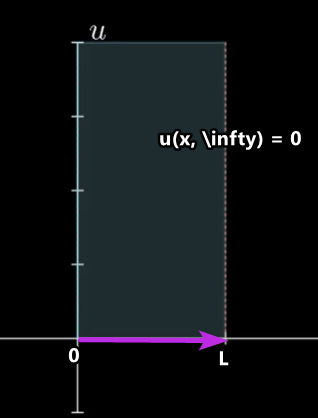
\includegraphics{FourierReflection}
\end{center}

So, whatever we get, we better have
$\displaystyle \lim_{t \to \infty} u(x, t) = 0$.
The method of reflection? relies on two things:

\begin{enumerate}
  \item Fourier Series
  \item Linearity
\end{enumerate}

\underline{Method}

\begin{enumerate}
  \item Try a solution of the form
  \begin{align}
    u(x, t) = X(x)T(t) \leftarrow \text{ Assume the solution is separable}
  \end{align}
  Boundary Conditions:
  Here, we conclude $X(0)$ is $0$ because
  we want $T(t)$ to change as $t$ changes.
  %
  \begin{align}
    u(0, t) = 0 & \Rightarrow X(0)T(t) = 0 \Rightarrow X(0) = 0\\
    u(L, t) = 0 & \Rightarrow X(L)T(t) = 0 \Rightarrow X(L) = 0\\
    U_t = \alpha^2 u_{xx} & \Rightarrow X(x)T^\prime(t) = \alpha^2 X^{\prime\prime}(x) T(t)
  \end{align}

  Here, we divide by $X, T, \alpha^2$.
  %
  \begin{align}
    \Rightarrow \frac{T^\prime(t)}{\alpha^2T(t)} & = \frac{X^{\prime\prime}}{X(x)} = -\lambda
  \end{align}

  Here, $\lambda$ is a constant.
  %
  \item
  \begin{align}
    \frac{X^{\prime\prime}}{X(x)} & = -\lambda\\
    X^{\prime\prime}(x) & = -\lambda X(x)
  \end{align}

  Here, we know $(x) = X(L) = 0$.
  We call every $(\lambda, X(x))$ pair that satisfies this equation
  an eigenvalue/eigenfunction pair for the differential equation.

  Assume $\lambda > 0$
  \begin{align}
    X^{\prime\prime} & = -\lambda x\\
    x(0) & = x(L) = 0\\
    & \Rightarrow X(x) = A \cos(\sqrt{\lambda} x) + B\sin(\sqrt{\lambda} x)\\
    & \Rightarrow A \cos 0 + B \sin 0 = 0\\
    & \Rightarrow A = 0\\
    & \Rightarrow X(x) = B \sin(\sqrt \lambda x)\\
    X(L) = 0 & \Rightarrow B \sin(\sqrt \lambda L) = 0\\
    & \Rightarrow \sin(\sqrt \lambda L) = 0\\
    & \Rightarrow \sqrt \lambda L = n \pi, n \in \Z^+\\
    & \Rightarrow \lambda_n = \Big( \frac{n \pi}{L} \Big)^2\\
    & \Rightarrow_n(x) = \FS
  \end{align}
\end{enumerate}

\topic{February 2, 2022}

\begin{align}
  u(x, t) & = X(x)T(t)\\
  \frac{X^{\prime\prime}}{x} & = \frac{T^\prime}{\alpha^2 T} = - \lambda\\
  \lambda_n & = \left( \frac{n \pi}{L} \right)^2\\
  X_n(x) & = \FS
\end{align}

Here, we have a basis function for Fourier Sine Series.

\begin{enumerate}
  \setcounter{enumi}{2}
  \item Solve for $T$
  \begin{align}
    \frac{T^\prime}{\alpha^2 T} & = - \lambda\\
    T^\prime & = -\alpha^2 \lambda T\\
    T^\prime_n & = - \alpha^2 \lambda_n T_n\\
    & = -\alpha^2 \left( \frac{n \pi}{L} \right)^2 T
  \end{align}
  If we have something like $y^\prime = ky$, we know that this derives from $y = e^{kx}$.
  \begin{align}
    T_n(t) & = e^{-\alpha^2 \left( \frac{n \pi}{L} \right)^2 T}
  \end{align}
  \item Combine for $u_n$
  \begin{align}
    u_n(x, t) & = X_n(x)T_n(t)\\
    & = \FS e^{-\alpha^2 \left( \frac{n \pi}{L} \right)^2 T}
  \end{align}

  Each one of the $n's$ will yield a different $u$. We also know that $n \in \N$. We can take as many $u'$s and add them all together. We find our $u_n'$s and use it to find $u$.

  By linearity,
  %
  \begin{align}
    u(x, t) & = \sum^\infty_{n = 1} A_n\\
    & = \sum^\infty_{n = 1} A_n \FS e^{-\alpha^2 \left( \frac{n \pi}{L} \right)^2 T}
  \end{align}

  \item Satisfy the initial condition
  \begin{align}
    u(x, 0) & = f(x)\\
    u(x, 0) & = \sum^\infty_{n = 1} A_n \FS = f(x)
  \end{align}
  Line 113) is considered the Fourier Sine Series.

  The $A_n'$s are the coefficients of the Fourier Sine Series of $f(x)$.
  \begin{align}
    A_n & = \frac{1}{L} \int^L_{-L} f(x) \FS dx\\
    & = \frac{2}{L} \int^L_0 f(x) \FS dx
  \end{align}
\end{enumerate}

\ex Solve with the following conditions:

\begin{enumerate}
  \item $u_t = 4u_{xx}$
  \item $u(0, t) = u(3, t) = 0$
  \item $u(x, 0) = 5 \sin \left( \frac{2 \pi x}{3} \right) - 7 \sin(4 \pi x)$
\end{enumerate}

Now, let us perform the five steps to solve our equation:

\begin{enumerate}
  \item Assume $u(x, t) = X(x)T(t)$\\
  Boundary Conditions :
  \begin{itemize}
    \item $u(0, t) = 0$, then $X(0)T(t) = 0$. Here either $X(0)$ or $T(t)$ is $0$, and we want $X(0) = 0$ here.
    \item $(3, t) = 0$, then $X(3)T(t) = 0$, following the same logic, we have $X(3) = 0$.
  \end{itemize}
  %
  \begin{align}
    u_t & = 4u_{xx}\\
    XT^\prime & = 4X^{\prime\prime}T\\
    \frac{T^\prime}{4T} & = \frac{X^{\prime\prime}}{X} = -\lambda
  \end{align}

  \item Now, since we know more information regarding $X$, let us solve for $X$.
  \begin{align}
    \frac{X^{\prime\prime}}{X} & = -\lambda\\
    X^{\prime\prime} & = -\lambda X, \quad X(0) = X(3) = 0
  \end{align}

  Let us assume $\lambda > 0$. Here, we want an $X^{\prime\prime}$ where deriving twice gives us $-X$. Assume $\lambda > 0$
  %
  \begin{align}
    X & = A\sin(\sqrt \lambda x) + B \cos(\sqrt \lambda x)
  \end{align}

  Set $X(0) = 0$
  %
  \begin{align}
    X & = A
  \end{align}

  Now, let us find $X(3) = 0$:
  %
  \begin{align}
    0 & = A\sin(\sqrt \lambda 3)\\
    \sqrt \lambda 3 & = n \pi\\
    \lambda_n & = \left( \frac{n \pi}{3} \right)^2\\
    X_n(x) & = \sin \left(\frac{n \pi x}{3} \right)
  \end{align}

  \item Now, let us find $T$.
  \begin{align}
    \frac{T^\prime}{4T} & = -\lambda\\
    T^\prime_n & = -4 \left( \frac{n \pi}{3} \right)^2 T_n\\
    T_n(t) & = e^{-4 \left( \frac{n^2 \pi^2}{9} \right)t}
  \end{align}
  %
  \item Combine to find $u_n$ and $u$
  \begin{align}
    u_n(x, t) & = X_n(x)T_n(t)\\
    & = \sin\left( \frac{n \pi x}{3} \right) e^{-4 \left( \frac{n^2 \pi^2}{9} \right)t}
  \end{align}

  By linearity,
  %
  \begin{align}
    u(x, t) & = \sum^\infty_{n = 1} A_n \sin\left( \frac{n \pi x}{3} \right) e^{-4 \left( \frac{n^2 \pi^2}{9} \right)t}
  \end{align}

  \item Use the initial conditions to find $A_n'$s
  \begin{align}
    u(x, 0) & = 5\sin(\frac{2 \pi x}{3}) - \sin(4 \pi x)\\
    u(x, 0) & = \sum^\infty_{n = 1} A_n \sin\left( \frac{n \pi x}{3} \right)\\
    A_n & = \frac{2}{3} \int^3_0 5 \left[\sin\left( \frac{2 \pi x}{3} \right)
    - 7 \sin(4 \pi x) \right] \sin(\frac{n \pi x}{3}) \dx
  \end{align}

  Lets look at our initial condition on line 133).
  The first one is $n =2$, so $A_2 = 5$.
  In addition, the second term is at $A_12 = -7$.
  Therefore, we have $A_n = 0 \forall n$ except $n = 2, 12$.

  Now, let us look at our linearity equation.
  %
  \begin{align}
    u(x, t)
    & = 5 \sin\left( \frac{2 \pi x}{3} \right)
    e^{-\frac{16 \pi^2}{9} t} - 7 \sin\left( 4 \pi x \right) e^{-64 \pi^2 t}
  \end{align}

  Here, this is our final solution.

  \subsection{Laplace's Equation}

  1-D : $u_{xx} = 0 \Rightarrow u = ax + b$

  If $u(0) = u(L) = 0$, then that would force our function to be $u = 0$. This is the steady state solution. If our function is in the form of $ax + b$, then $u = 0$ is the only solution for the function to hit $0$ twice in this fashion.

  2-D: $\Delta u = 0 \Rightarrow u_{xx} + u_{yy} = 0$

  \begin{center}
    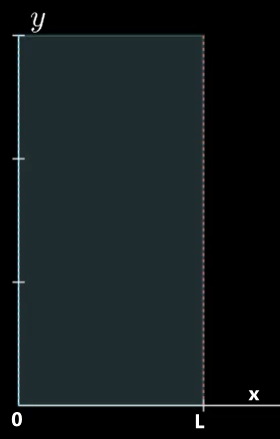
\includegraphics{Laplaces}
  \end{center}

  We have two types of boundary conditions:
  %
  \begin{enumerate}
    \item Specify $u$ on the perimeter
    \begin{itemize}
      \item $u(0, y) = 0$
      \item $u(L, y) = 0$
      \item $u(x, 0) = 0$
      \item $u(x, M) = f(x)$
    \end{itemize}
    \item Nuemann conditions :
    Specify the direction derivative in the normal direction on the boundary.
    \begin{itemize}
      \item $u_x(0, y) = 0$
      \item $u_x(L, y) = 0$
      \item $u_y(x, 0) = 0$
      \item $u_y(x, M) = \twiddle{f}(x)$
      \item $u(0, 0)\  = T$
    \end{itemize}
    This is if we know the heat flux $\vec q \cdot \vec n$ on the boundary.
  \end{enumerate}
\end{enumerate}

\bigbreak

\subsection{Solving Laplace's Equation}

\topic{February 4, 2022}
\begin{center}
  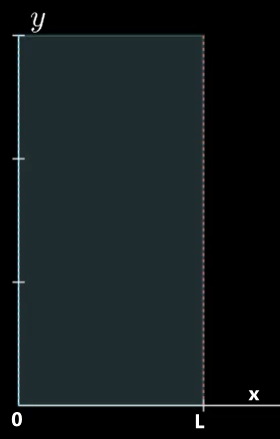
\includegraphics{Laplaces}

  $u_{xx} + u_{yy} = 0$
\end{center}
%
\begin{itemize}
  \item $u_x(0, y) = 0$
  \item $u_x(L, y) = 0$
  \item $u(x, 0) = 0$
  \item $u(x, M) = f(x)$
\end{itemize}
%
\begin{enumerate}
  \item Assume $u(x, y) = X(x)Y(y)$

  \underline{Boundary Conditions}
  \begin{align}
    u(x, y) & = X(x) Y(y)\\
    & \Rightarrow X^\prime(x)Y(y)
  \end{align}

  Now, let us write our boundary condition:
  %
  \begin{align}
    U_x(0, y) & = 0\\
    & \Rightarrow X^\prime(0)Y(y) = 0\\
    & \Rightarrow X^\prime(0) = 0
  \end{align}

  Now, let us find the next item,
  %
  \begin{align}
    u_x(L, y) & = 0\\
    & \Rightarrow X^\prime(L)Y(y) = 0\\
    & \Rightarrow X^\prime(L) = 0
  \end{align}

  Now, the next two items do not have a derivative:
  %
  \begin{align}
    u(x, 0) & = 0\\
    & \Rightarrow X(x)Y(0) = 0\\
    & \Rightarrow Y(0) = 0
  \end{align}

  Now, let us write:
  %
  \begin{align}
    u_{xx} + u_{yy} & = 0\\
    & \Rightarrow X^{\prime\prime}Y + XY^{\prime\prime} = 0\\
    & \Rightarrow X^{\prime\prime}Y = - XY^{\prime\prime}\\
    & \Rightarrow \frac{X^{\prime\prime}}{X} = - \frac{Y^{\prime\prime}}{Y}
    = -\lambda
  \end{align}

  \item Solve for $X$
  (Note: We solve for $X$ first here, since we have more information about $X$).
  %
  \begin{align}
    \frac{X^{\prime\prime}}{X} & = - \lambda\\
    \Rightarrow X^{\prime\prime}
    & = - \lambda X, \quad X^\prime(0) = X^\prime(L) = 0\\
    \lambda > 0 \Rightarrow x(x)
    & = A \sin(\sqrt \lambda x) + B \cos(\sqrt \lambda x)\\
    \Rightarrow X^\prime(x)
    & = A \sqrt \lambda \cos(\sqrt \lambda x)
    - B \sqrt \lambda \sin(\sqrt \lambda x)\\
    X^\prime(0) = 0 \Rightarrow A \sqrt \lambda & = 0
  \end{align}

  Now, if we rewrite out equation, we have:

  \begin{align}
    X(x) & = B \cos(\sqrt \lambda x)
  \end{align}

  Next, we want to find $X^\prime(L) = 0$:
  %
  \begin{align}
    0 & = - B \sqrt \lambda \sin(\sqrt \lambda L)\\
    \sqrt \lambda L & = n \pi\\
    \lambda_n & = \left(\frac{n \pi}{L}\right)^2\\
    \Rightarrow X_n(x) & = \FC
  \end{align}

  If $\lambda = 0$
  %
  \begin{align}
    \frac{X^{\prime\prime}_0}{X_0} & \Rightarrow X^{\prime\prime}_0 = 0\\
    & \Rightarrow X_0(x) = Ax + B\\
    & \Rightarrow X^\prime_0(x) = A\\
    & \Rightarrow X^\prime_0(0) = 0\\
    & \Rightarrow A = 0\\
    & \Rightarrow X^\prime_0(L) = 0\\
    & \Rightarrow A = 0
  \end{align}

  Neither conditions tell us more information about $B$,
  %
  \begin{align}
    \Rightarrow X_0(x) = B_0
  \end{align}

  \item Now, we want to solve for $Y$: $- \frac{Y^{\prime\prime}}{Y} = -\lambda$
  \begin{align}
    Y^{\prime\prime} & = \lambda y\\
    Y^{\prime\prime} & = \left( \frac{n \pi}{L} \right)^2 Y_n, \quad Y_n(0) = 0\\
    Y_n(y) & = Ce^{\frac{n \pi}{L}y} + De^{- \frac{n \pi}{L}}y\\
    Y_n(0) = 0 & \Rightarrow C + D = 0
  \end{align}

  Here, we do not have an additional condition that could help use
  solve this equality. Let us consider the hyperbolic sin and cos:
  %
  \begin{align}
    \sinh(x) & = \frac{e^x - e^{-x}}{2}\\
    \cosh(x) & = \frac{e^x + e^{-x}}{2}
  \end{align}

  Instead of writing $Y$ in the same fashion we solved for $X$,
  we use the hyperbolic $\sinh$ and $cosh$
  %
  \begin{align}
    Y_n(y) & = C \sinh \left(\frac{n \pi y}{L} \right)
    + D \cosh \left( \frac{n \pi y}{L} \right)\\
    Y_n(0) = 0 & \Rightarrow D = 0\\
    Y_n(y) & = \sinh \left( \frac{n \pi y}{L} \right)
  \end{align}

  Now, let us write:
  %
  \begin{align}
    \frac{Y^{\prime\prime}_0}{Y_0} = \lambda_0 &\\
    & \Rightarrow Y^{\prime\prime}_0 = 0\\
    & \Rightarrow Y_0 = Cy + D\\
    & \Rightarrow Y_0(0) = 0\\
    & \Rightarrow D = 0\\
    & \Rightarrow Y_0(y) = C_0 y
  \end{align}

  \item Combine to find $u_n$ and $u$:
  \begin{align}
    u_n(x, y) = X_n(x)Y_n(y) & =
    \begin{cases}
      \FC \sinh \left( \frac{n \pi y}{L} \right) & n \geq 1\\
      B_0C_0y & n = 0
    \end{cases}
  \end{align}

  By linearity,
  %
  \begin{align}
    u(x, y) & = \twiddle{B}_0 y
    + \sum^\infty_{n = 1} B_n \FC \sinh \left( \frac{n \pi y}{L} \right)
  \end{align}

  \item Here, use the final boundary condition to find the coefficients.
  \begin{align}
    u(x, M) & = f(x)\\
    u(x, M) & = \twiddle{B}_0
    M + \sum^\infty_{n = 1} B_n \FC \sinh\left( \frac{n \pi M}{L} \right)
  \end{align}

  This is our Fourier Cosine Series for $f(x)$.
  Here, we can say a few things about this equation,
  %
  \begin{itemize}
    \item $b_0 = \twiddle B_0 M$
    \item $b_n = B_n \sinh\left( \frac{n \pi M}{L} \right)$
  \end{itemize}
  %
  \begin{align}
    \twiddle B_0 M & = \frac{2}{2L} \int^L_0 f(x) \dx\\
    \twiddle B_0 & = \frac{1}{ML} \int^L_0 f(x) \dx
  \end{align}

  Next, let us find:
  %
  \begin{align}
    B_n \sinh\left( \frac{n \pi M}{L} \right)
    & = \frac{2}{L} \int^L_0 f(x) \FC \dx\\
    & = \frac{2}{L \sinh\left( \frac{n \pi M}{L} \right)} \int^L_0 f(x) \FC \dx
  \end{align}
\end{enumerate}

\ex Solve $\Delta u = 0$
%
\begin{itemize}
  \item $(x, y) = 0$
  \item $(2, y) = 0$
  \item $(x, 0) = 0$
  \item $(x, 3) = 4 \sin (5x)$
\end{itemize}
%
\begin{enumerate}
  \item Assume $u(x, y) = X(x)Y(y)$

  Here, let us look at our boundary conditions:
  %
  \begin{align}
    u(0, y) & = 0\\
    X(0)Y(y) & = 0\\
    X(0) = 0
  \end{align}

  Here, let us look at our next boundary conditions:
  %
  \begin{align}
    u(2, y) & = 0\\
    X(2)Y(y) & = 0\\
    X(2) = 0
  \end{align}

  Here, let us look at our next boundary conditions:
  %
  \begin{align}
    u(x, 0) & = 0\\
    X(x)Y(0) & = 0\\
    Y(x) = 0
  \end{align}

  Now, we can write:
  %
  \begin{align}
    u_{xx} + u_{yy} & = 0\\
    X^{\prime\prime}Y + XY^{\prime\prime} & = 0\\
    \frac{X^{\prime\prime}}{X} & = -\frac{Y^{\prime\prime}}{Y} = - \lambda
  \end{align}
  %
  \item Now, let us solve for $x$:
  \begin{align}
    \frac{X^{\prime\prime}}{X} & = -\lambda\\
    X^{\prime\prime} & = - \lambda X, \quad X(0) = X(2) = 0\\
    \lambda > 0 \Rightarrow X(x)
    & = A \sin(\sqrt \lambda x) + B \cos(\sqrt \lambda x)\\
    X(0) & = B = 0\\
    X(2) & = A \sin(\sqrt \lambda 2) = 0\\
    & = \lambda 2 = n \pi\\
    & = \lambda_n = \left( \frac{n \pi}{2} \right)^2\\
    & = X_n(x) =  \sin(\frac{n \pi x}{2})
  \end{align}

  \item Let us solve for $y$:
  \begin{align}
    \frac{Y^{\prime\prime}_n}{Y_n} & = \lambda_n\\
    Y^{\prime\prime}_n
    & = \left(\frac{n \pi}{2}\right)^2 Y_n, \quad Y_n(0) = 0\\
    Y_n(y)
    & = C \sinh \left( \frac{n \pi y}{2} \right)
    + D \cosh \left( \frac{n \pi y}{2} \right)\\
    & = Y_n(0) = 0 \Rightarrow D = 0\\
    Y_n(y) & = \sinh \left( \frac{n \pi y}{2} \right)
  \end{align}

  We are picking a constant for this last term later, so we can drop $C$.
\end{enumerate}

Here, let us write out our equation for the following function,

\topic{February 7, 2022}
\begin{itemize}
  \item $\Delta u = 0$
  \item $u(0, y) = 0$
  \item $u(2, y) = 0$
  \item $u(x, 0) = 0$
  \item $u(x, 3) = 4$
  \item $\lambda_n = \left(\frac{n \pi}{2}\right)^2$
  \item $X_n(x) = \sin\left(\frac{n \pi x}{2}\right)$
  \item $Y_n(x) = \sinh\left(\frac{n \pi y}{2}\right)$
\end{itemize}

\begin{enumerate}
  \setcounter{enumi}{3}
  \item Combine to find $u_n$ and $u$
  \begin{align}
    u_n(x, y)
    & = \sin\left( \frac{n \pi x}{2} \right)\sinh\left(\frac{n\pi y}{2} \right)
  \end{align}

  By linearity,
  %
  \begin{align}
    u(x, y)
    & = \sum^\infty_{n = 1}
    A_n \sin\left( \frac{n \pi x}{2} \right)
    \sinh\left( \frac{n \pi y}{2} \right)
  \end{align}

  \item Find coefficients using last boundary conditions
  \begin{align}
    u(x, y)
    & = 4 \sin(5 \pi x)\\
    u(x, y)
    & = \sum^\infty_{n = 1}
    A_n \sin\left(\frac{n \pi x}{2} \right)
    \sinh\left(\frac{n \pi 3}{2} \right)\\
    & = 4\sin(5 \pi x)
  \end{align}

  Recall, the coefficient of the Fourier Sine Series is anything but $\sin$.
  Notice our last line with discrete number,
  our coeficient must equal $4$ and our $n$ is 10, therefore, we write:
  %
  \begin{align}
    A_{10} \sinh\left( \frac{10 \pi 3}{2} \right) & = 4\\
    \Rightarrow A_{10} & = \frac{4}{\sinh(15 \pi)} % ?
  \end{align}
\end{enumerate}
